\section{Results and discussion}
The number of fringes was plotted against the pressure change for the different gases and is found in Fig. \ref{fig:measurements}. As one can see in the figures all gases showed a linear relation which was expected. When comparing Fig. \ref{fig:Helium} with the others the number of fringes is a lot lower than for the others. This means that the index of refraction must be a lot lower for this and the relative error will probably be larger. It also means that the relative error in the result will be quite larger in this result in comparison to the others.

The linear fit parameters are found in Tab. \ref{tab:linearFits}. As expected, the slope $a$ for helium is a lot lower than the other slopes. From these slopes, the refractive indexes was Calculated using Eq. \eqref{eq:slope} and tabulated in Tab. \ref{tab:refrIndex}.

\begin{figure}[H]
  \centering
  \begin{subfigure}{0.49\textwidth}
    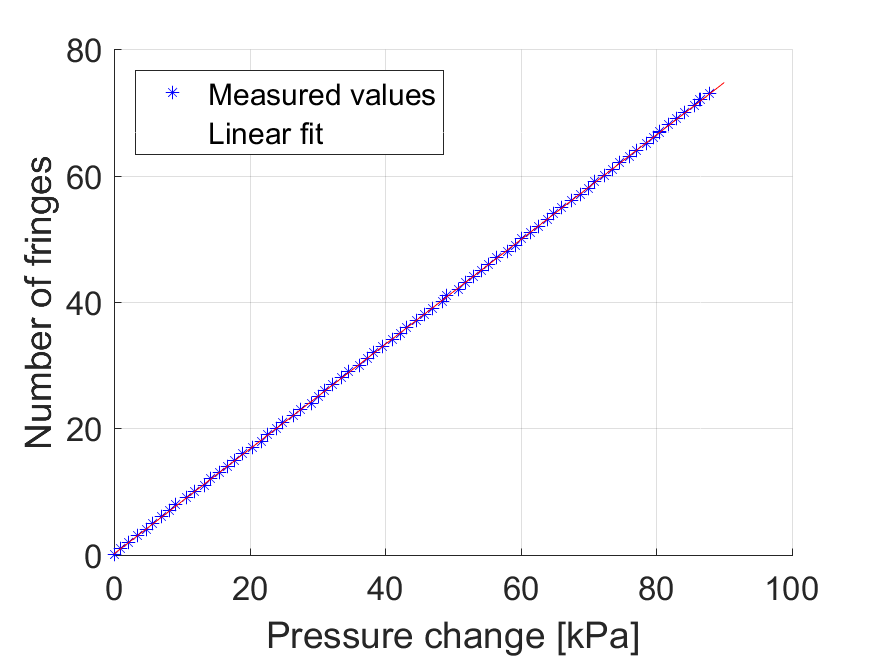
\includegraphics[width=\textwidth]{matlab/Air}
    \caption{Air}
    \label{fig:Air}
  \end{subfigure}
  \begin{subfigure}{0.49\textwidth}
    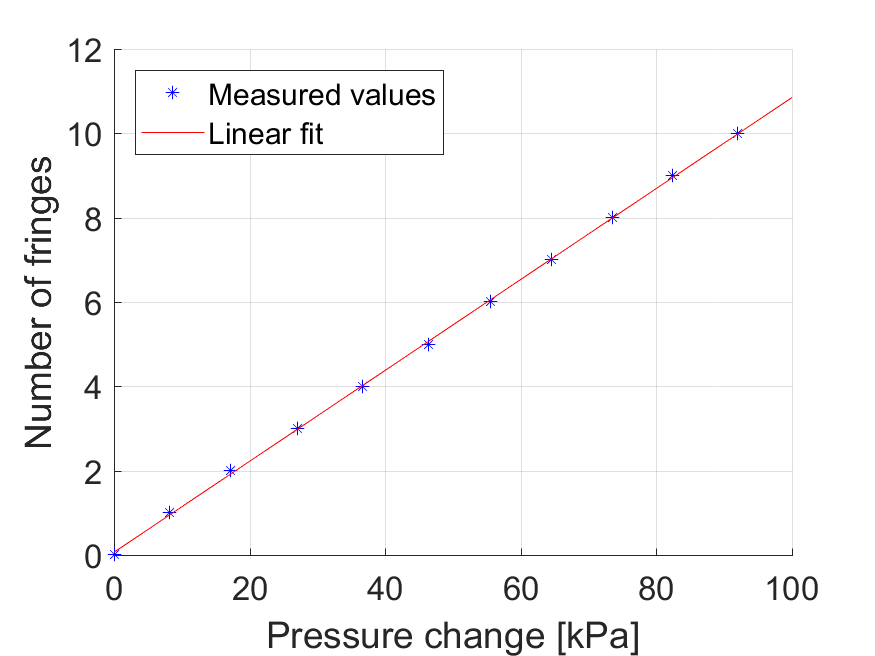
\includegraphics[width=\textwidth]{matlab/Helium}
    \caption{Helium}
    \label{fig:Helium}
  \end{subfigure}
  \begin{subfigure}{0.49\textwidth}
    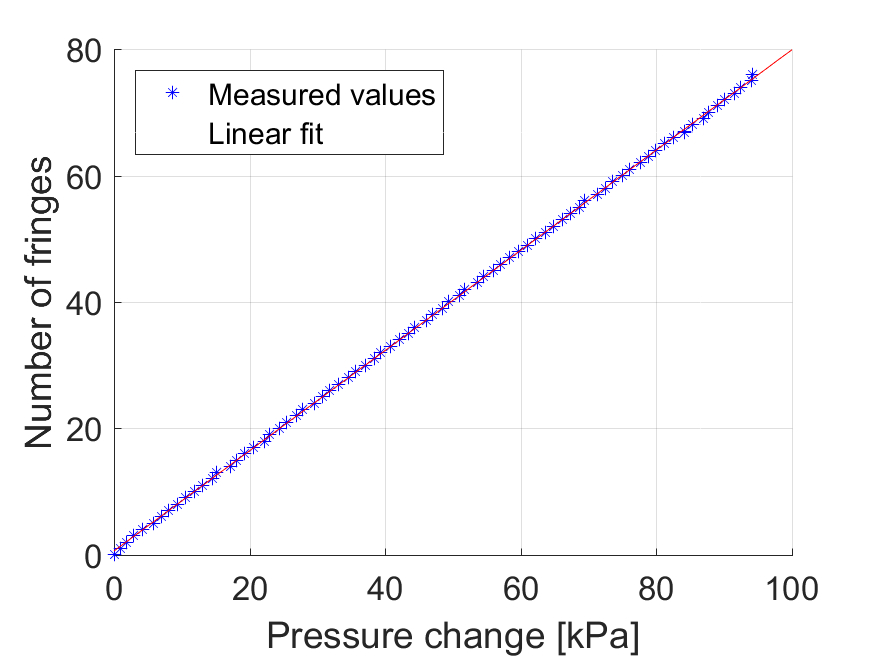
\includegraphics[width=\textwidth]{matlab/Argon}
    \caption{Argon}
    \label{fig:Argon}
  \end{subfigure}
  \begin{subfigure}{0.49\textwidth}
    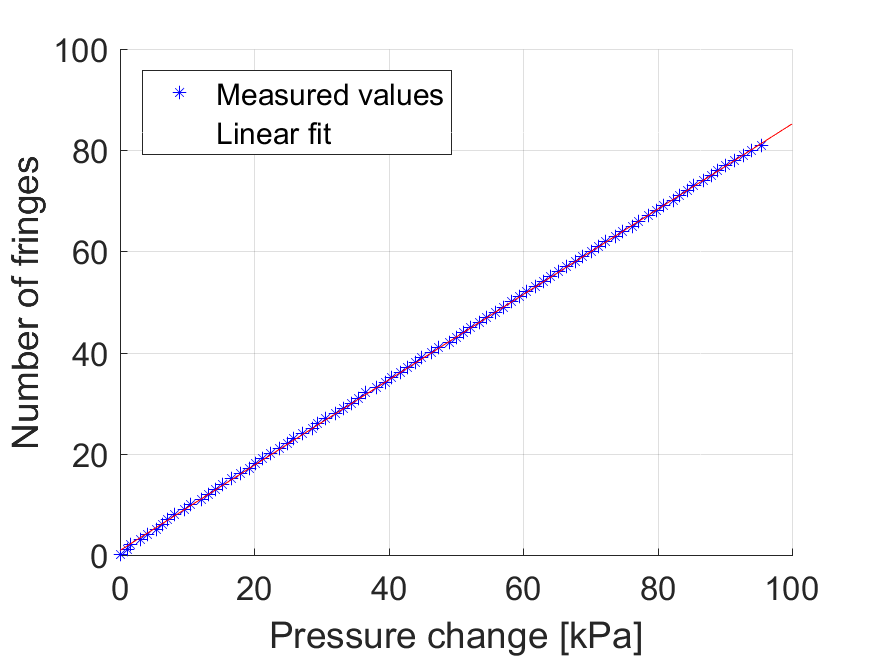
\includegraphics[width=\textwidth]{matlab/Nitrogen}
    \caption{Nitrogen}
    \label{fig:Nitrogen}
  \end{subfigure}
  \caption{Number of fringes and pressure change for the different gases with linear fits. Fitting parameters are found in Tab. \ref{tab:linearFits}}
  \label{fig:measurements}
\end{figure}

\begin{table}[H]
  \centering
  \caption{Fitting parameters for the measured values in Fig. \ref{fig:measurements}. Linear fit on the form $y=\alpha x + \beta$.}
  \label{tab:linearFits}
  \begin{tabular}{l|l|l}
           & $\alpha$ [kPa$^{-1}$]& $\beta$ \\ \hline
  Air      & $0.83(2)$  & $0.16(6)$ \\
  Helium   & $0.11(1)$ & $0.06(5)$ \\
  Argon    & $0.79(3)$ & $0.61(5)$ \\
  Nitrogen & $0.84(2)$ & $0.86(5)$
  \end{tabular}
\end{table}

\begin{table}[H]
  \centering
  \caption{Estimated refractive indexes for the gases including tabulated values}
  \label{tab:refrIndex}
  \begin{tabular}{l|l|l}%|l}
          & Calculated & Tabulated  \\ \hline %& Error \\ \hline
    Air      & $1.000264(6)$  & $1.000271$ \cite{idxAir} \\ %& $7.05654305 \cdot 10^{-6}$ \\
    Helium   & $1.000034(4)$  & $1.000032$ \cite{idxHeli} \\ %& $2.07707264 \cdot 10^{-6}$ \\
    Argon    & $1.000253(9)$  & $1.000261$ \cite{idxArg} \\ %& $8.23800429 \cdot 10^{-6}$ \\
    Nitrogen & $1.000269(6)$  & $1.000276$ \cite{idxNit} \\ %& $7.55338923 \cdot 10^{-6}$
  \end{tabular}
\end{table}

As seen in the table the tabulated refractive indexes are inside the error margin for helium and argon and slightly outside for air and nitrogen. Notice that the relative error is wastly larger for helium than for the others since its refractive index is much lower. This is due to that there was a lot fewer data points for this gas, as seen in Fig. \ref{fig:Helium}. Note also that the calculated values are lower that the tabulated values for all gases but helium indicating that there might be a systematic error that is unknown. One reason for this could be that the measurements was not started from perfect vaccum. The pump that was used to generate vaccum only achieved about 0.2-0.4kPa of pressure which intruduces a shift of the measurements. Since the refractive index at this pressure is still approximatly one in Eq. \ref{eq:refrInd}, only the right hand side would shift which would introduce a slightly higher slope. Then question then would be why the refracted index of helium was higher. This could be due to that the lack of measurements overtake this error in the opposite direction.

%All the tabulated values for index of refraction is within the calculated ones error of margin, as seen in Tab. \ref{tab:refrIndex}. The major thing to notice from the results is that the error margin for helium is approximatly five times larger than the errors for the other gases. This is expected, since helium generated only $10$ fringes while the other gases generated about $70-80$ fringes (i.e. alot more).


